\begin{frame}
\begin{block}{me}
In the early 2000s, I was working for IBM, on the Java Development Kit \ldots
\end{block}
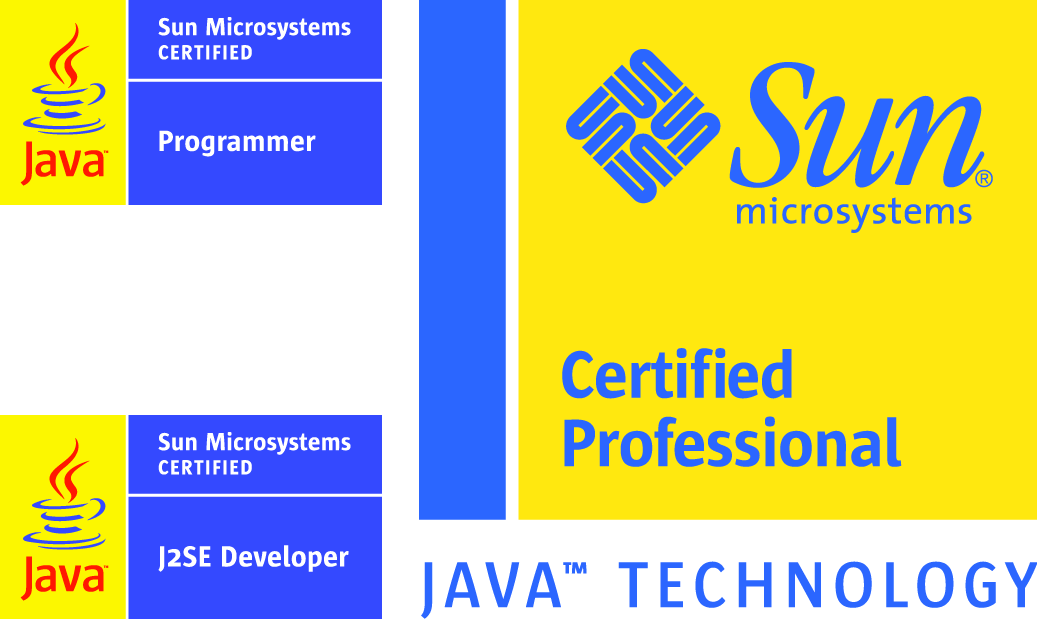
\includegraphics[height=1.2cm]{image/java-certs.png}
\end{frame}

\begin{frame}
\begin{block}{me}
navigating the principles of software engineering, I had one simple thought \ldots
\end{block}
\end{frame}

\begin{frame}
\begin{block}{me}
\begin{quote}
surely there is a better way and someone smarter than me has figured it out
\end{quote}
\end{block}
\end{frame}

\begin{frame}
\begin{block}{me}
I learned that yes, sound and applicable principles for software engineering have been figured out
\end{block}
\end{frame}

\begin{frame}
\begin{block}{me}
It is called Functional Programming
\end{block}
\end{frame}
